\section{Experiments}

\subsection{Experimental Setup}
\label{sec:exp_setup}

\paragraph{Models and Datasets} 
We primarily evaluate our method using the Qwen2.5-Instruct~\citep{Qwen2.5} series, ToolLLaMA~\citep{Qin:2024toolllm} series, LLaMA-3.1-8B-Instruct, and LLaMA-3.2-3B-Instruct~\citep{llama3}. The evaluation covers four widely used tool-use benchmarks: API-Bank~\citep{apibank}, ToolAlpaca~\cite{ToolAlpaca}, BFCLv2~\cite{BFCL}, and ToolBench~\cite{Qin:2024toolllm}. Additional details of these datasets are provided in the Appendix~\ref{appendix:dataset_details}.

\paragraph{Implementation Details} 
The retrieval parameter $k$ is set to 10. For suffix matching, we follow PLD~\citep{saxena2023pld} and consider suffix lengths $L \in \{5,6,7\}$. The continuations are extracted using predefined lengths $n \in \{32, 16, 8, 8\}$. We adopt Token Recycling (TR)~\citep{luo:2025tokenrecycle} as the general speculative strategy in \method. Following prior work, we adopt speculative sampling~\citep{leviathan:2023spec} as our acceptance strategy, with a batch size of 1. Additional implementation details are provided in the Appendix~\ref{appendix:impl_details}.

\paragraph{Baselines} 
We primarily compare \method to three existing \textit{plug-and-play} methods: PLD~\citep{saxena2023pld}, TR~\citep{luo:2025tokenrecycle}, and SAM-Decoding (SAMD)~\citep{hu2025:samd}. For SAMD, we construct the static SAM from the input context and adopt TR as its decoding strategy. For comparison, we also include the advanced training-required methods Eagle-2~\citep{li2024:eagle2} and Eagle-3~\citep{li2025:eagle3} in our main results.

\begin{figure}[t]
\centering
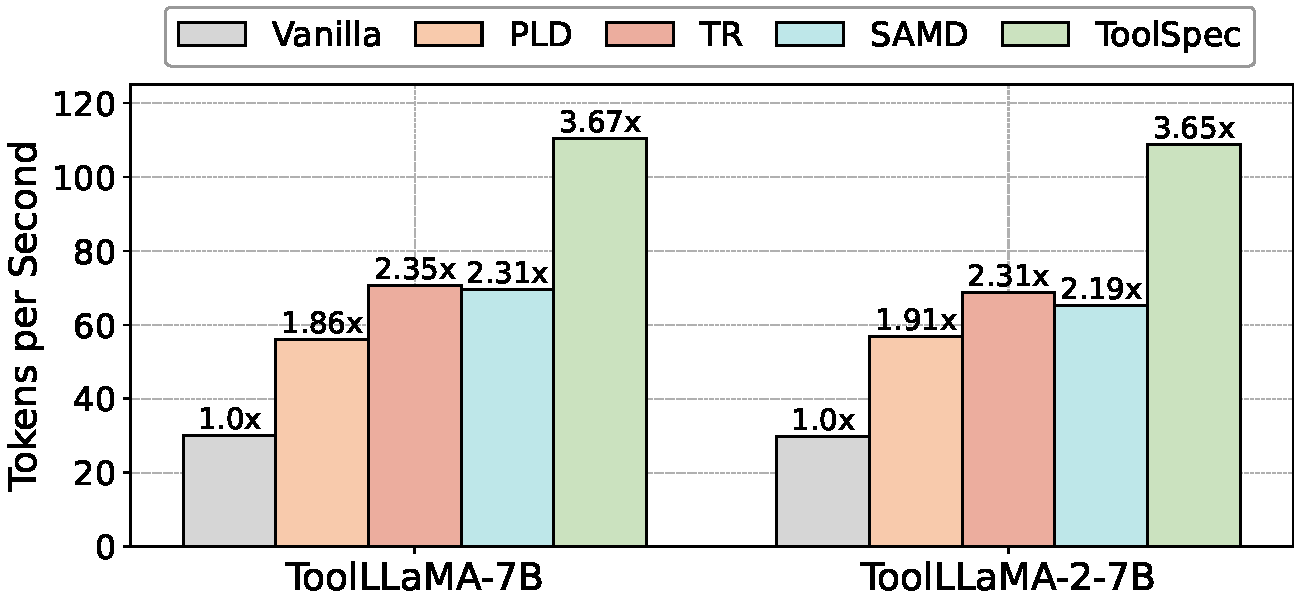
\includegraphics[width=0.95\columnwidth]{fig/toolllama.pdf}
\caption{Speedup comparison between \method and prior plug-and-play methods on ToolBench.}
\vspace{-0.5cm}
\label{fig:toolllama}
\end{figure}

\paragraph{Evaluation Metrics} 
We evaluate \method using three widely adopted metrics: the mean number of accepted tokens (\#MAT), throughput (tokens/s), and wall-clock speedup relative to vanilla autoregressive decoding. From a theoretical perspective, \method preserves the output distribution of the target LLM, thereby obviating the need for extensive evaluation of generation quality. Nevertheless, we report performance on API-Bank and ToolAlpaca in Appendix~\ref{appendix:performance} for reference.

\subsection{Main Results} 
Table~\ref{tab:main-exp} compares the inference efficiency of \method with prior plug-and-play methods on widely used tool-use tasks. The results reveal the following key findings: (1) \method consistently outperforms existing approaches, achieving speedups of $3.5\times$$\sim$$4.2\times$ over standard autoregressive decoding across a range of models and tasks. Compared with the previous best method, it yields up to a $\bf{71\%}$ relative improvement in speedup (from $2.45\times$ to $4.19\times$). (2) The efficiency gains of \method are primarily attributed to a high number of accepted tokens (denoted as \#MAT), ranging from $4.02$ to $5.80$ across different settings. Unlike model-based SD methods such as Eagle-3, \method does not require an additional drafting module and introduces only minimal drafting overhead (approximately $6\%$, as shown in Figure~\ref{fig:profile}). This low overhead enables the increased \#MAT to translate more effectively into end-to-end speedup.

\paragraph{Discussion on Eagle Performance}
We observe that the \#MAT achieved by the Eagle series is lower than that of prior plug-and-play methods, such as TR, as shown in Table~\ref{tab:main-exp}. We hypothesize that this gap arises because Eagle models are not trained on tool-calling formats, making such inputs out-of-distribution for these models. In contrast, as discussed in Section~\ref{sec:pattern_analysis}, tool-calling traces exhibit structural regularities and recurring invocation patterns. These properties favor SD methods such as TR, which leverage historical traces to construct draft sequences. Building on this insight, \method exploits the schema-constrained nature of tool-calling tasks, enabling more accurate draft generation and achieving higher overall efficiency.

\paragraph{Results on ToolLLaMA}
In addition to general-purpose LLMs, we further evaluate \method on two variants of ToolLLaMA, a model specifically trained for tool-use tasks. Figure~\ref{fig:toolllama} presents a comparison of inference efficiency between \method and prior plug-and-play SD methods on ToolBench. The results show that \method achieves a speedup of approximately $3.7\times$ over standard autoregressive decoding, demonstrating its effectiveness on specialized tool-use LLMs.